\Chapter{Példák játékosításra épülő alkalmazások}

A fejezet bemutatja, hogy milyen, a dolgozat későbbi fejezeteiben bemutatásra kerülő alkalmazáshoz hasonló kész szoftverek érhetők el. Ezek technikai értelemben véve szintén alkalmazások, viszont a köréjük épült ökoszisztéma miatt már szolgáltatásoknak tekinthetjük őket.

\Section{Problémakör}

A legtöbb rendszer magára a funkcionalitásra fókuszál, hogy elvégezzünk rajta egy meghatározott tevékenységet a lehető leggyorsabban. Ami munkavégzés szempontjából hatékony, viszont a fogyasztó úgy fogja érezni, hogy neki ezt azért kell csinálni mert muszáj, nem azért mert szükségszerűen el akarják látni azt a bizonyos feladatot. \newline

Ezzel ellentétben az emberközpontú tervezést alkalmazó rendszerek használatakor nem érezzük úgy magunkat, hogy az emberek egy kis fogaskerekek egy nagy rendszerben. Az emberközpontú tervezés arra optimalizál, hogy motivációs hatása legyen, elkötelezettséget váltson ki belőlünk, természetesen az elvégzendő feladat mellett. A valóság az, hogy a munkával ellentétben játszani nem kötelező, ha nem tetszik egy játék bármelyik pillanatban abba lehet hagyni. Emiatt ember központúak a játékok mert a játék készítőinek muszáj lefoglalnia a játékost, ezért van az a sok küldetés, cél és évtizedek alatt kitapasztalt rengeteg játékos elem, hogy a játékos ne hagyja abba a játékot \cite{actionablegamification}.

\Section{Elérhető alkalmazások}

Napjainkban a két legelterjedtem alkalmazást választottam mintául a saját alkalmazásom elkészítéséhez. Az egyik ilyen alkalmazás a \textit{Duolingo} \cite{duolingo} a másik pedig a \textit{Kahoot!} \cite{kahoot}. Mind a kettőt az oktatást játékosítására hozták létre.

\SubSection{Kahoot!}

A Kahoot! tömören egy olyan tanulási platform, amelyen egyszerűen lehet létrehozni, megosztani és kitölteni kvízeket. \newline

De ahhoz, hogy elkészítsük őket először regisztrálni kell, lehet tanár, diák, személyes vagy szakmai fiókot létrehozni. Miután ez megvan, akkor elkezdhetjük az oldal használatát. \newline

A kvíz készítési része az oldalnak egyszerű, letisztult és intuitív, könnyen lehet kérdéseket hozzáadni és szerkeszteni. Ki tudjuk választani, hogy milyen formában szeretnénk számon kérni a felhasználót. Négy válaszlehetőség közül lehet választani egy jót vagy szimplán igaz/hamis állítást feltenni.

Ennek a kiválasztása után megírhatjuk magát a kérdést és a négy válaszlehetőséget, kijelölhetjük melyik a jó válasz. Tudunk beállítani minden kérdéshez idő limitet, hogy hány pontot érjen a kérdésre a helyes válasz, egy vagy több jó válasz legyen, valamint milyen képet szeretnénk a kérdéshez illeszteni (\ref{fig:kahoot_1}. ábra).

\begin{figure}[h!]
	\centering
	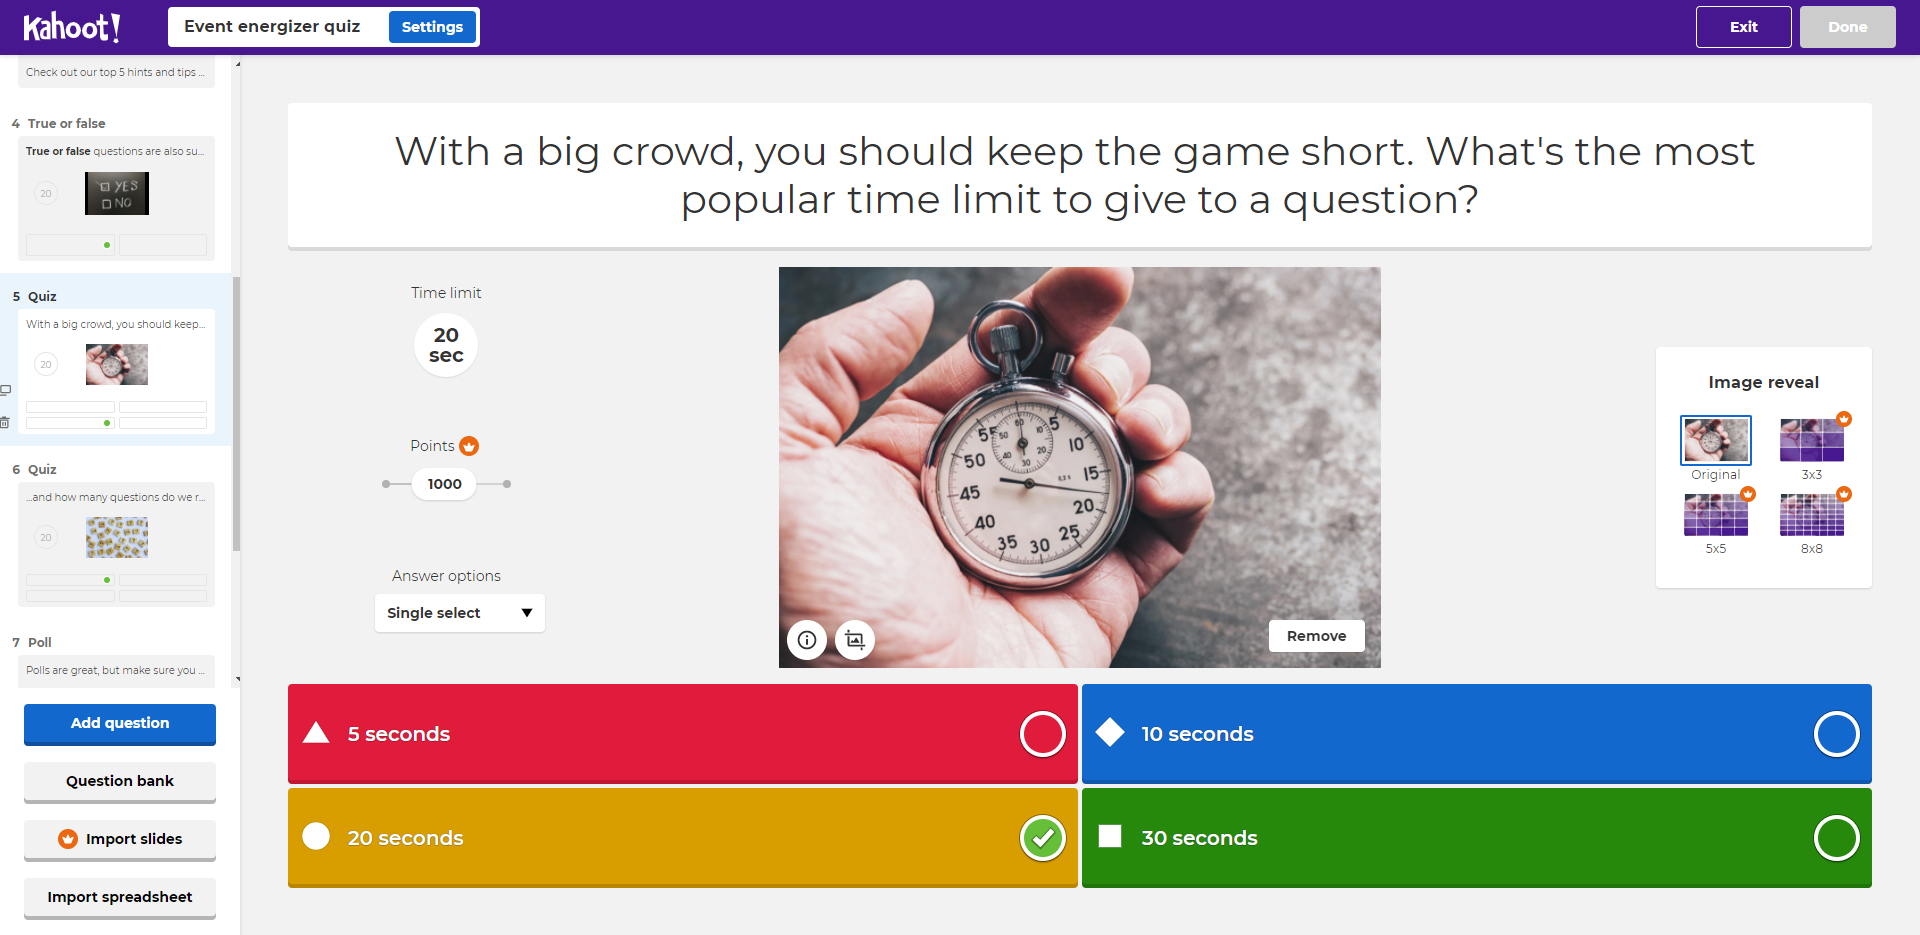
\includegraphics[width=\linewidth]{images/kahoot_test_making.PNG}
	\caption{Teszt készítése Kahoot!-on}
	\label{fig:kahoot_1}
\end{figure}

Amint kész vagyunk, akkor mások is kitölthetik a tesztünket. Ezt úgy lehet elérni, hogy elkészítés után generálódik egy PIN amit a felhasználó beír és már csatlakozhat is. Amennyiben minden felhasználó csatlakozott akkor a teszt készítője elindíthatja a játékot és a játékosok egyszerre látják a kérdéseket, saját eszközeiken pedig válaszolhatnak rájuk (\ref{fig:kahoot_2}. ábra).

\begin{figure}[H]
	\centering
	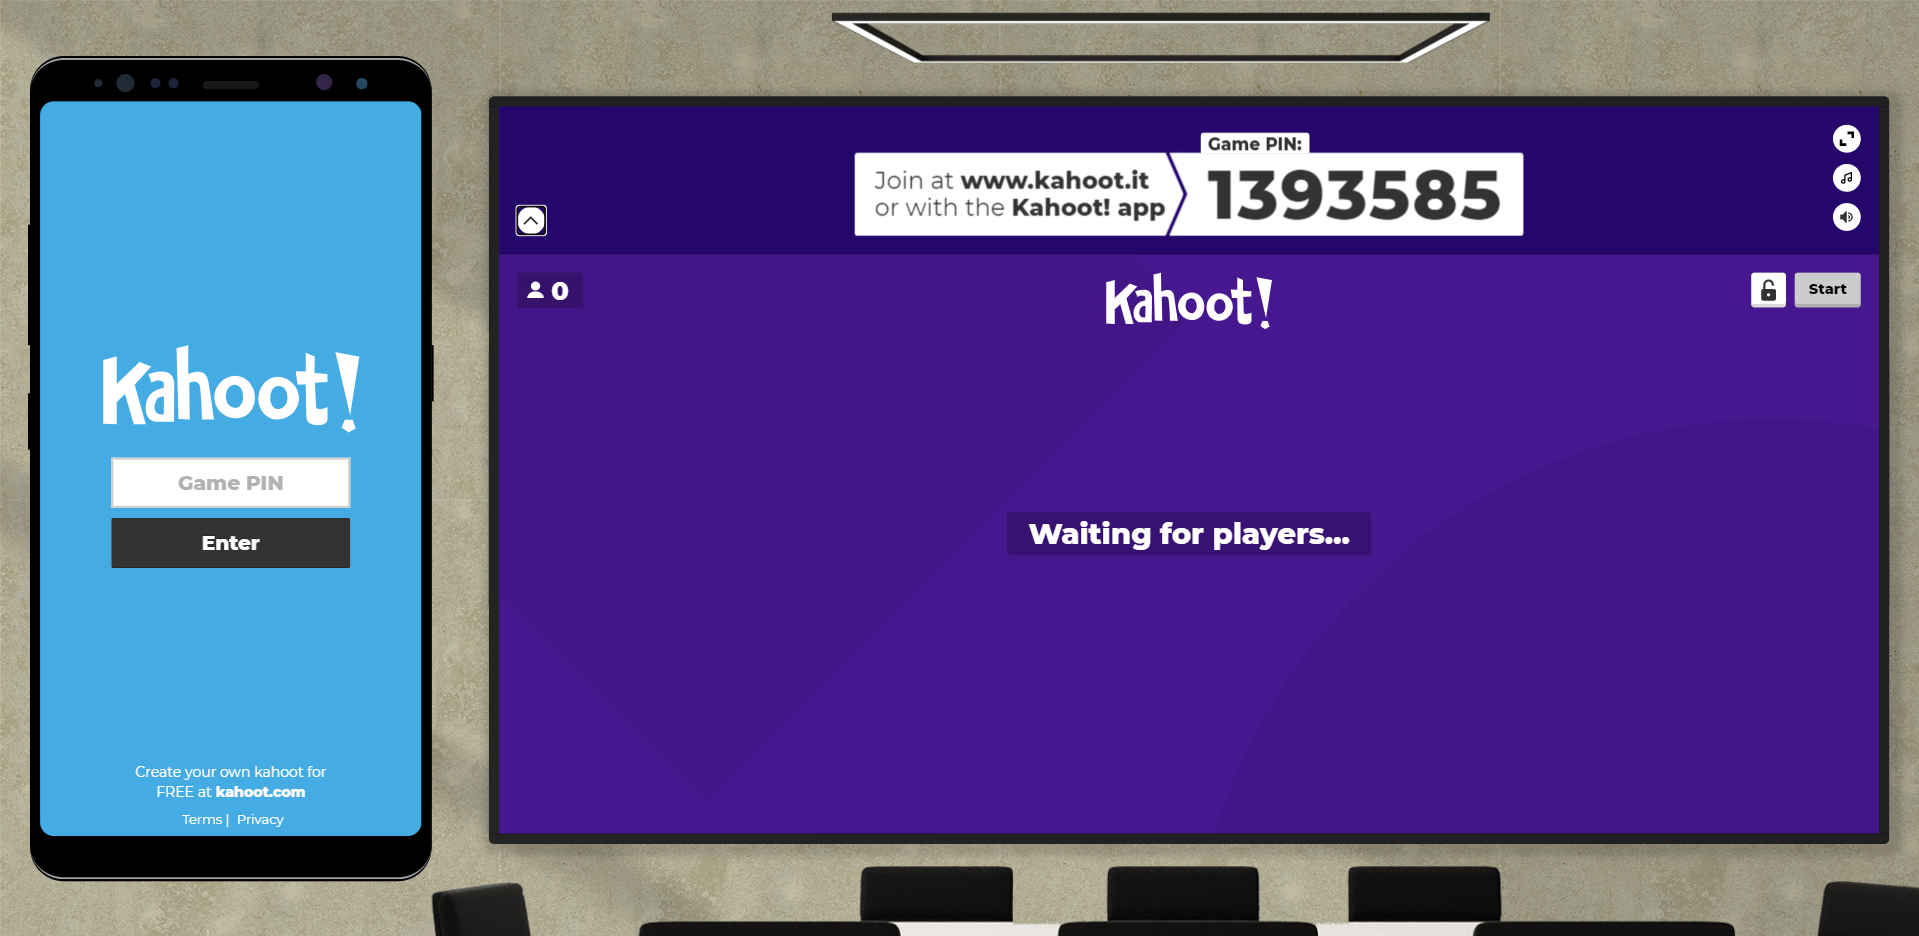
\includegraphics[width=\textwidth]{images/kahoot_play.png}
	\caption{Várakozás játékosokra Kahoot!-on}
	\label{fig:kahoot_2}
\end{figure}

A kérdések után láthatjuk mennyien válaszoltak az adott válaszra, és ezek közül melyik volt a korrekt. Mi magunk pedig látjuk, helyes volt-e a megadott válaszunk és mennyi pontot szereztünk. Majd a kérdéssorozat után láthatjuk az első három helyezettet és pontjaikat. A játék késztője egy teljes jelentést nézhet meg a játszott felhasználók teljesítményéről (\ref{fig:kahoot_3}. ábra).

\begin{figure}[h]
	\centering
	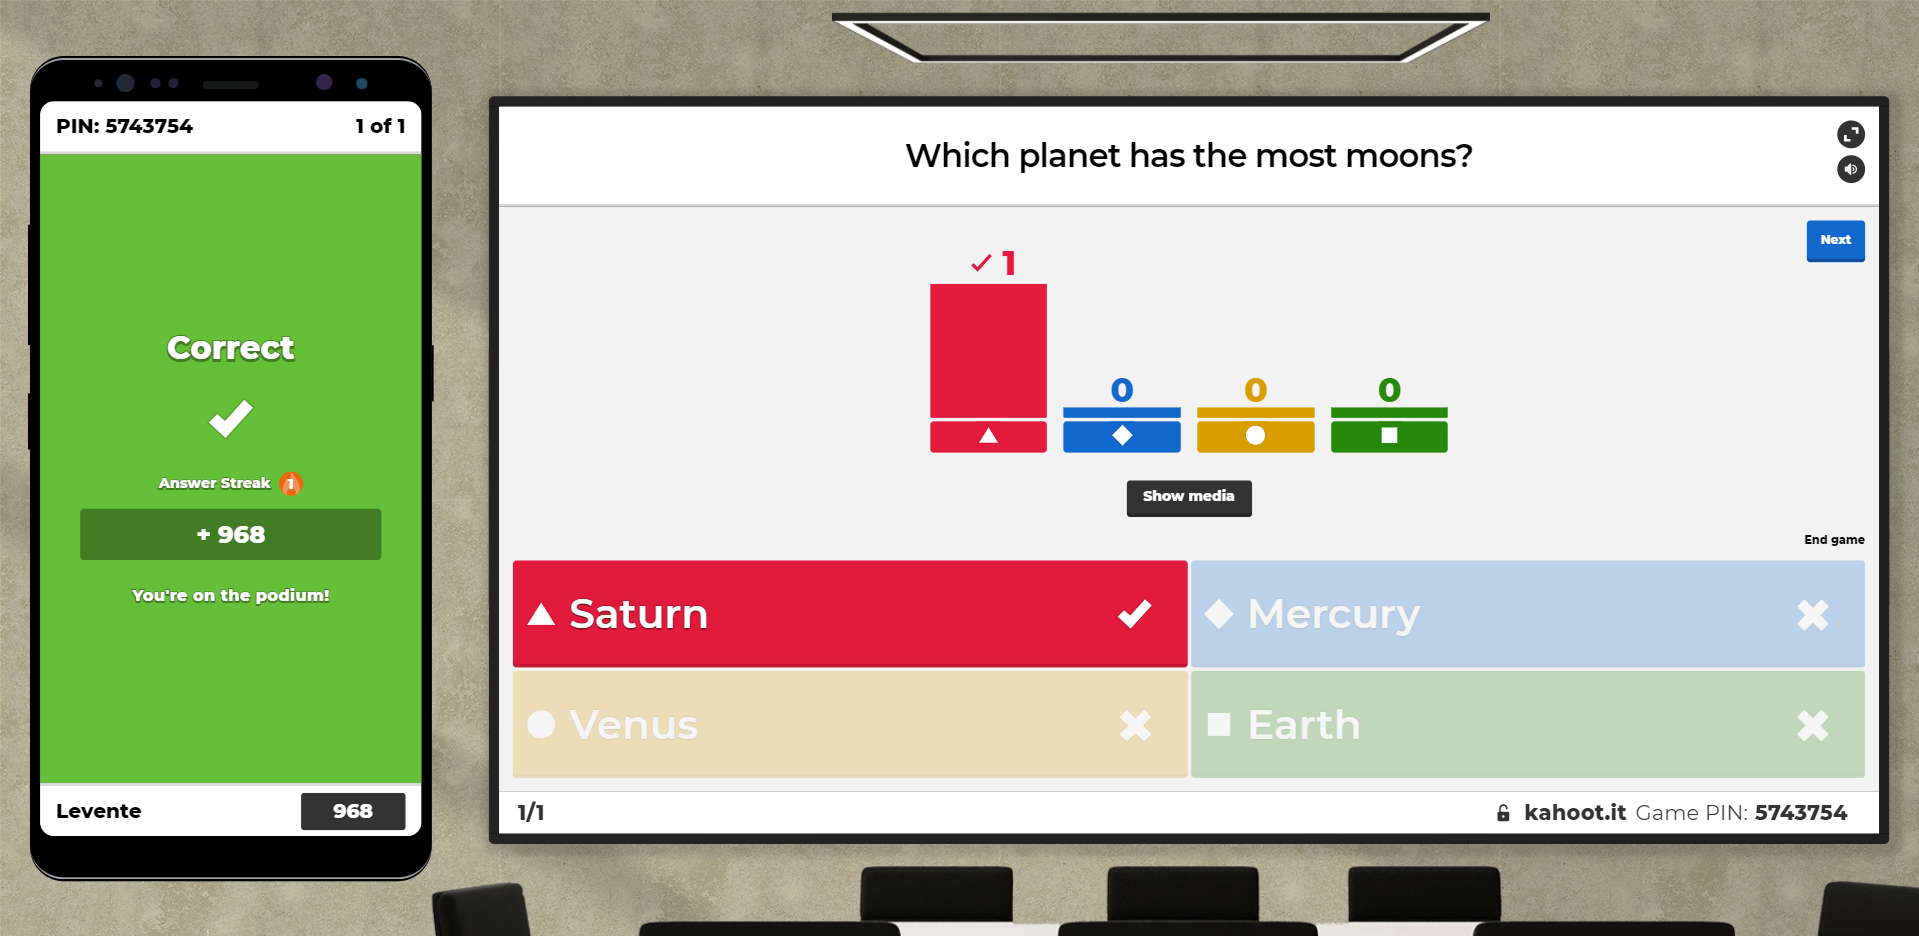
\includegraphics[width=\textwidth]{images/kahoot_play2.png}
	\caption{Válaszadás Kahoot!-on}
	\label{fig:kahoot_3}
\end{figure}

\SubSection{Duolingo}

A Duolingo a legnépszerűbb nyelvtanulási platform és a legtöbbet letöltött oktatási alkalmazás a világon, több mint 300 millió felhasználóval. Az alkalmazás célja az oktatás ingyenes, szórakoztató és mindenki számára elérhetővé tétele. A Duolingo-t úgy tervezték, hogy úgy érezze a felhasználó, hogy egy játékkal játszik \cite{whatIsDuolingo}.
\Aref{fig:duolingo}. ábrán láthatunk egy képet a webalkalmazásról.

\begin{figure}[h]
  \centering
  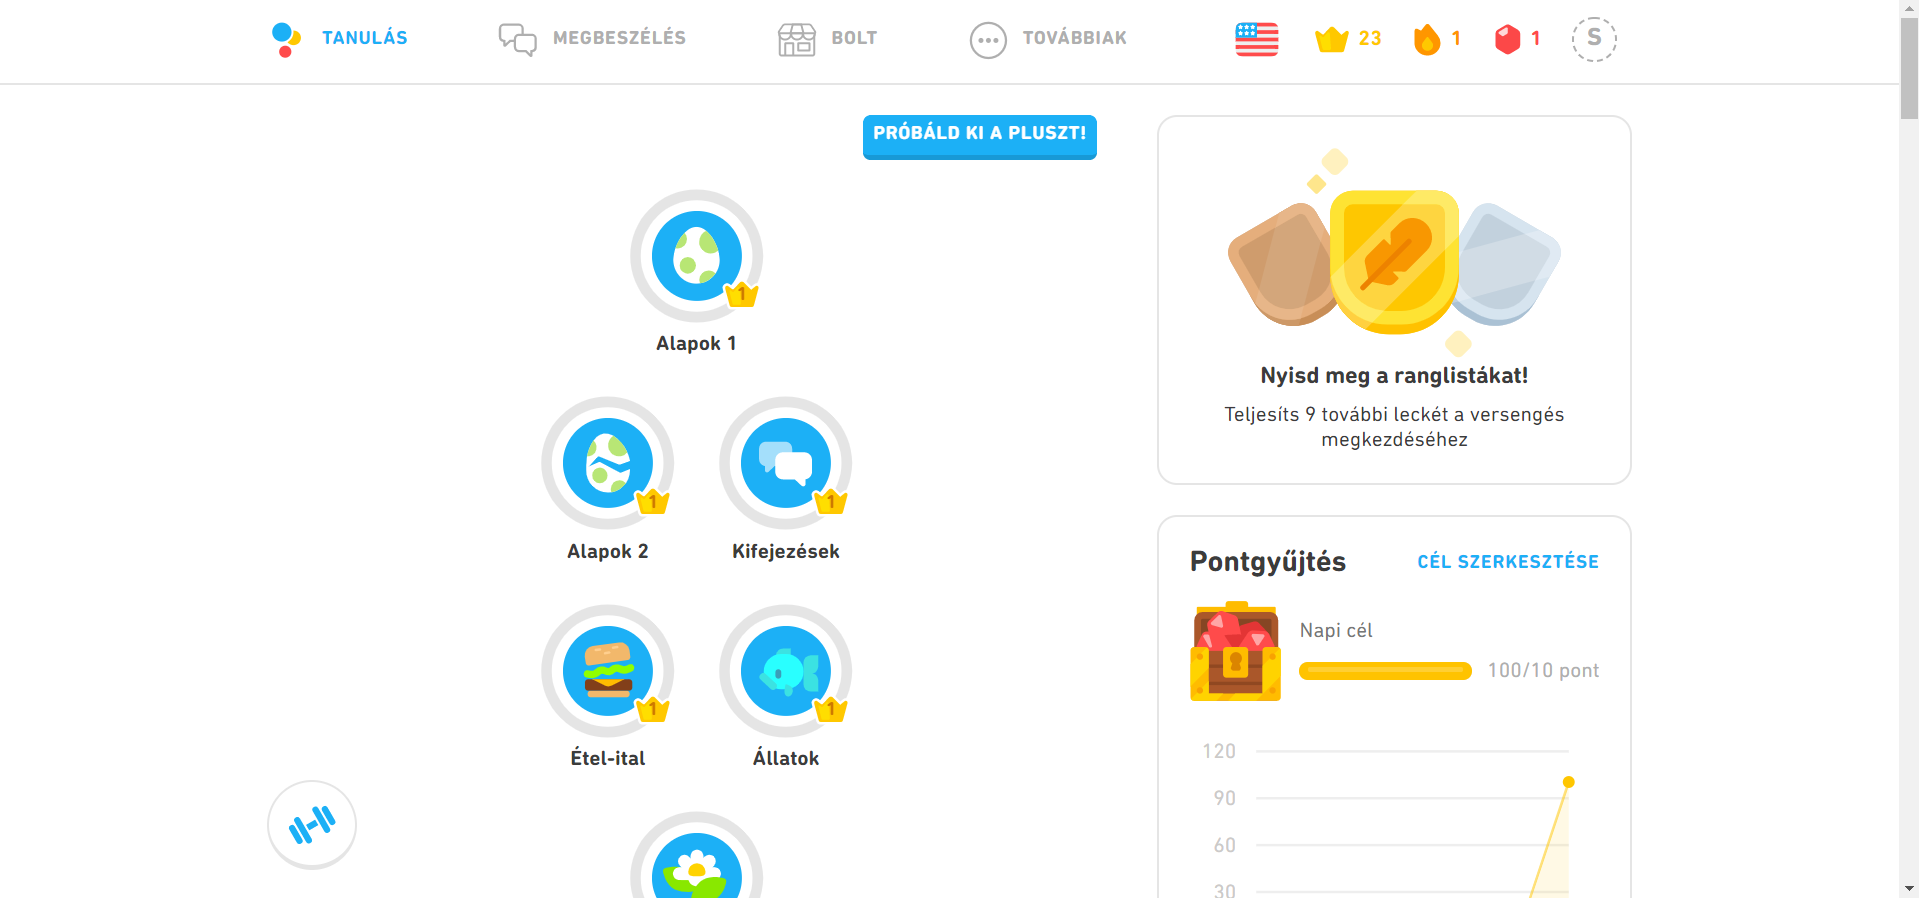
\includegraphics[width=\textwidth]{images/Duolingo_main_page.png}
  \caption{Egy kép a Duolingo-ról}
  \label{fig:duolingo}
\end{figure}

A felületen is már látható a játékosság megjelenése és a játékokból vett elemek megléte. Például:
\begin{itemize}
  \item {Pontgyűjtés}
        \begin{addmargin}[\parindent]{0pt}
          Tanulás során pontokat lehet szerezni, amelyeket tapasztalati pontoknak neveznek. Erre leckék elvégzésével, ismeretanyag gyakorlásával vagy például szintugró-teszt elvégzésével van lehetőség.
        \end{addmargin}
  \item Napi cél
        \begin{addmargin}[\parindent]{0pt}
          A napi cél a motiváció megőrzésére szolgál. Beállíthatjuk, hogy naponta hány pontot szeretnénk szerezni tanulással. A napi jutalmat akkor lehet megkapni, amikor teljesíti a felhasználó a kitűzött célt.
        \end{addmargin}
  \item Koronák
        \begin{addmargin}[\parindent]{0pt}
          Minden ismeretanyaghoz tartozik egy koronaszint. A felhasználó, hogy ha szintet lép egy ismeretből, akkor Koronát szerez, és a feladatok egyre nehezebbek lesznek. Dönthet úgy, hogy mélyebben beleássa magát egy ismeretanyagba, és megpróbál magasabb szintre jutni, vagy egy új ismeretanyagot is megnyithat, hogy új tartalmakat tanulhasson \cite{koronaszintekDuolingo}.
        \end{addmargin}
  \item Széria
        \begin{addmargin}[\parindent]{0pt}
          A széria a napok számát jelzi amelyek során minden egymást követő napon elvégzésre került egy lecke. Miután befejeztük a leckét az alkalmazásban vagy a weboldalon, a széria 1 nappal növekszik. Egy kis tűz ikon jelképezi a szériát. Amíg el nem érjük a napi célt, az szürkén jelenik meg, a napi lecke elvégzése után pedig színessé válik \cite{szeriaDuolingo}.
        \end{addmargin}
  \item Barátok
        \begin{addmargin}[\parindent]{0pt}
          Lehetnek az alkalmazáson belül barátaink, akiknek megnézhetjük az elért eredményeit és követhetjük egymást, ezáltal láthatjuk a másik fejlődését.
        \end{addmargin}
  \item Ranglista
        \begin{addmargin}[\parindent]{0pt}
          A ranglista egy olyan elem, amely segítségével versenyezhetünk a többi nyelvtanulóval egy ligán belül. Pontokat lehet szerezni és ezáltal feljutni a ranglista csúcsára. Ezután a ranglistán szereplő tíz legjobban teljesítő felhasználó a következő héten magasabb szintre lép. Az utolsó tíz versenyző, pedig az előző szintre kerül vissza.
        \end{addmargin}
\end{itemize}

\Section{Eddigi eredmények felhasználása}

A saját alkalmazásomba bele szeretném vinni előzőleg bemutatott mindkét alkalmazásból a következő elemeket: \textit{tesztkészítés}, \textit{pontgyűjtés}, \textit{ranglista}.
